\documentclass[a4paper,12pt]{article}

\usepackage{authblk}
\usepackage[margin=1.5in]{geometry}
\usepackage{setspace}
\usepackage[T1]{fontenc}
\usepackage{calc}
\usepackage[hyphens]{url}

\usepackage{amsmath}

\usepackage[mono=false]{libertine}
\usepackage{unicode-math}
\setmathfont[Scale=MatchUppercase]{libertinusmath-regular.otf}

\usepackage{inconsolata}
\setmonofont{inconsolata}

\usepackage{color}
\definecolor{lightgray}{gray}{0.9}
\usepackage{listings}
\lstset{language=R, keywordstyle=\color{black}, basicstyle=\ttfamily\small,backgroundcolor = \color{lightgray}, frame=trbl, rulecolor=\color{black}, framesep=10pt}

\usepackage{pifont}
\usepackage{hhline}
\usepackage{booktabs}
\usepackage{longtable}
\setlength{\LTleft}{0pt}
\usepackage{colortbl}
\usepackage{gb4e-}
\usepackage{graphicx}
\usepackage{mdframed}
\usepackage{hyperref}

\usepackage{boxedminipage2e}

\usepackage[backend=biber,
	natbib=true,
	style=bst/unified/bbx/biblatex-sp-unified,
	citestyle=bst/unified/cbx/sp-authoryear-comp,
	maxbibnames=99,
	isbn=false,
	doi=false,
	eprint=false
]{biblatex}

\newcommand{\Lf}{
  \setlength{\itemsep}{1pt}
  \setlength{\parskip}{0pt}
  \setlength{\parsep}{0pt}
}

\newcommand{\wrt}{w.\,r.\,t.\ }
\newcommand{\ie}{i.\,e.,\ }
\newcommand{\Ie}{I.\,e.,\ }
\newcommand{\eg}{e.\,g.,\ }
\newcommand{\Eg}{E.\,g.,\ }
\newcommand{\Aa}{The author\ }
\newcommand{\A}{the author\ }
\newcommand{\Sub}[1]{\ensuremath{\mathrm{_{#1}}}}
\newcommand{\Sup}[1]{\ensuremath{\mathrm{^{#1}}}}
\newcommand{\Subsf}[1]{\ensuremath{\mathsf{_{#1}}}}
\newcommand{\Supsf}[1]{\ensuremath{\mathsf{^{#1}}}}
\newcommand{\pPB}{p\Subsf{PB}}
\newcommand{\mpPB}{\ensuremath{p_{\text{PB}}}}
\newcommand{\vivs}{VI\slash VS\ }

\bibliography{rs,cow}

\title{Mixed-effects regression modeling}
\author{Roland Schäfer}
\affil{Freie Universität Berlin}
\date{\today}

\setlength\parindent{0pt}
\doublespacing

\begin{document}       

\maketitle

\section{Introduction}
\label{sec:introduction}

Mixed effects modeling -- alternatively called \textit{hierarchical} or \textit{multilevel modeling} is a straightforward extension of (generalized) linear modeling as discussed in the previous chapter.
A common characterization of mixed-effects modeling is that it accounts for situations where observations are \textit{clustered} or \textit{come in groups}.
In corpus linguistics, there could be clusters of observations defined by individual speakers, registers, genres, modes, lemmas, etc.
Instead of estimating a coefficients for each level of such a grouping factor (a so-called \textit{fixed effects}), in a mixed model they can be modeled as normally distributed random variable (a so-called \textit{random effect}) with predictions being made for each group.
This chapter introduces the situations where mixed-effects modeling is useful, including a discussion of the alternative models without random effects.
The proper specification of models without and with R are discussed, as well as some model diagnostics and ways of interpreting the output.
Readers are assumed to be familiar with the concepts covered in the previous chapter.

\section{Fundamentals}
\label{sec:fundamentals}

\subsection{When are random effects useful?}
\label{sec:whenrandomeffectsareuseful}

\subsubsection{Introduction to random effects}
\label{sec:introductiontorandomeffects}

% \textit{Generalized Linear Models} (GLMs), as discussed in the previous chapter, allow us to estimate the effects which various \textit{predictors} or \textit{regressors} (\ie corpus linguistic variables) have on an \textit{outcome} or \textit{response} (\ie another corpus linguistic variable).
% Surely, the most typical application (in corpus linguistics) is the modeling of \textit{alternations}, \ie phenomena where the response variable of interest encodes a choice of forms or constructions, for example a case alternation (a binary or multi-valued categorical response), alternations of graphemic forms such as contracted vs.\ non-contracted, ordering preferences such as the order of prenominal adjectives, or syntactic\slash constructional alternations such as the dative alternation.%
% \footnote{In this article, I restrict the discussion to GL(M)Ms with categorical responses, simply because the continuous responses in Linear (Mixed) Models -- or LM(M)s – are not found very often in corpus linguistics.
% Also, an L(M)M can be understood as a GL(M)M with an identity link function and a Gaussian distribution for the residuals.}
% The approach is called \textit{generalized} in contrast to normal linear models because the response need not be numerical, and the \textit{errors} or \textit{residuals} do not have to be (approximately) normally distributed.
% First, this is achieved by allowing for different types of exponential distributions for the residuals, which requires the use of a more general estimator than least-squares, typically likelihood maximization.
% Second, \textit{link functions} are introduced which relate the additive linear term that combines the predictors in a non-linear way to the response variable.
(Generalized) Linear Mixed Models (GLMMs) are an extension of (Generalized) Linear Models.
They add what are often called \textit{random effects} and \textit{mix} them with the normal predictors (\textit{fixed effects}) as used in GLMs.
Alternatively, statisticians speak of \textit{multilevel models} or \textit{hierarchical models} \citep{GelmanHill2006}, a terminology to be explained in Section~\ref{sec:hierarchicalormultilevelmodels}.

The purpose of including random effects is usually said to be the modeling of variance between groups of observations.
A single observation (or \textit{data point} or \textit{measurement} or \textit{unit}) is one atomic exemplar entering into the statistical analysis of the study.
In corpus linguistics, single observations can be understood as a single line in a concordance, and they typically represent, for example (and with reference to the above examples), a clause or sentence in which one of the alternants of a case alternation occurs, an NP where two pre-nominal adjectives are used, a single occurrence of a contracted or non-contracted form, etc.
When such observations are grouped, it is often plausible to assume that some variance in the choice of the alternating forms or constructions occurs at the group-level and not at the level of observations.
If this is the case and the grouping factor is not included in the model, the error terms within the groups will be correlated.
Since the estimator works under the assumption of non-correlated errors, standard errors for model coefficients can be estimated as smaller than they nominally are, leading to increased Type I error rates in inferences about the coefficients.%
\footnote{Type I errors occur when the null hypothesis is rejected although it is true.}
This gets even worse when there are within-group tendencies regarding the direction and strength of the influence of the other regressors, \ie when there is an interaction between them and the grouping factor (\eg \citealt{SchielzethForstmeier2009}).
This is why known variation by group should always be accounted for in the model, and random effects are often a convenient way to do so.

Groups can be defined by any linguistically relevant grouping factor, such as the individual speakers (or authors, writers, etc.), their sex and gender, the regions where they were born or live, social groups with which they identify, but also time periods, genres, styles, etc.
% If the concordance in a study contains, say, ten exemplars each written by ten speakers, then the speaker grouping factor has ten levels and defines ten groups.
We know that preferences vary between speakers, and it is therefore reasonable to take care of this variance in our statistics in some way.
% The same goes for the other possible groups just mentioned.
Furthermore, it is known that specific lexemes often have idiosyncratic affinities towards alternants in alternating constructions.
Therefore, exemplars containing specific lexemes also constitute groups.
%  with considerable between-group variance.
% As an example from outside corpus linguistics, variation between participants is modeled by including a random effect for speaker in experimental settings.

% While random effects are often presented like this using conceptual arguments,
The crucial question in specifying models is not whether to include these grouping factors at all, but rather whether to include them as fixed effects or as random effects.
Random effects structures are very suitable for accounting for group-level variation in regression, but while formulaic recommendations such as ``Always include random effects for speaker and genre!'' provide useful guidance, the choice between fixed and random effects can and should be made based on an analysis and understanding of the data set at hand and the differences and similarities in the resulting models.
The remainder of Section~\ref{sec:whenrandomeffectsareuseful} introduces three important points to consider about the structure of the data typically used in mixed modeling.
% This is intended to show readers that mixed or multilevel\slash hierarchical modeling is simply a matter of doing justice to the structure of the data.
Then, Section~\ref{sec:modelspecificationandmodelingassumptions} provides a moderately technical introduction to modeling.
Section~\ref{sec:specifyingmodelsusinglme4inr} then shows how mixed models are specified using the \texttt{lme4} package in R, and Section~\ref{sec:afterfittingmodelswithlme4} deals with the interpretation of the output.


\subsubsection{Crossed an nested effects}
\label{sec:crossedandnestedeffects}

\begin{table}
  \centering
  \begin{tabular}{lll}
    \toprule
    \textbf{Exemplar} & \textbf{Speaker}  & \textbf{Region}        \\
    \midrule
                    1 &           Daryl  &         Tyneside       \\
                    2 &           Daryl  &         Tyneside       \\
                    3 &           Riley  &         Tyneside       \\
                    4 &           Riley  &         Tyneside       \\
                    5 &           Dale   &         Greater London \\
                    6 &           Dale   &         Greater London \\
                    7 &           Reed   &         Greater London \\
                    8 &           Reed   &         Greater London \\
    \bottomrule
  \end{tabular}
  \caption{Illustration of nested factors}
  \label{tab:nested}
\end{table}

% It was established in the previous section that random effects are a means of accounting for group-level variance in regression models.
% This section briefly introduces a distinction that plays a role in modeling when there is more than one grouping factor (to be used either as a fixed or random effect).
This section discusses a distinction that arises when there is more than one grouping factor.
When this is the case, each pair of grouping factors can be \textit{nested} or \textit{crossed}.
By way of example, we can group exemplars (such as sentences) by the individual speakers who wrote or uttered them, and we can group speakers by their region of birth.
Such a data set would intrinsically be \textit{nested}, as Table~\ref{tab:crossed} illustrates.
Since speakers have a unique region of birth, Tyneside is the unique region value for the speakers Daryl and Riley, and Greater London is the unique region value for Dale and Reed.
% There cannot be exemplars where, for example, the speaker is Daryl and the region is Greater London (assuming that speakers are uniquely identified by the labels in the middle column).
In this example, the region factor nests the speaker factor.
This example was chosen because the nesting is conceptually necessary.
However, even when a data set has a nested structure by accident, standard packages in R will treat them as nested
%, and a closer look at data sets should be part of any protocol for using GLMMs in corpus studies
(see Section~\ref{sec:specifyingmodelsusinglme4inr}).

When the grouped entities (themselves groups) do not uniquely belong to levels of the grouping factor, the factors are \textit{crossed}.
Continuing the example, crossed factors for speaker and mode are illustrated in Table~\ref{tab:crossed}.
%
\begin{table}
  \centering
  \begin{tabular}{lll}
    \toprule
    \textbf{Exemplar} & \textbf{Speaker}  & \textbf{Mode}   \\
    \midrule
                    1 &           Daryl  &         Spoken  \\
                    2 &           Daryl  &         Written \\
                    3 &           Riley  &         Spoken  \\
                    4 &           Riley  &         Spoken  \\
                    5 &           Dale   &         Written \\
                    6 &           Dale   &         Written \\
                    7 &           Reed   &         Spoken  \\
                    8 &           Reed   &         Written \\
    \bottomrule
  \end{tabular}
  \caption{Illustration of crossed factors}
  \label{tab:crossed}
\end{table}
%
While there are only spoken sentences by Riley and only written sentences by Dale in the sample, there is one spoken and one written sentence each by Daryl and Reed.
There is a many-to-many relation between speakers and modes, which is characteristic of crossed factors.
In Table~\ref{tab:nested}, the relation between speakers and regions was many-to-one, which is typical of nested factors.
% In experimental settings, the design often makes sure that the combinations of nested or crossed factors are represented by equal numbers of observations (such that, for example, there is an equal number of written and spoken sentences from each speaker).
% Contrarily, the situation in Table~\ref{tab:crossed} is typical of corpus studies where pseudo-random sampling from a pre-compiled corpus such as the BNC was used.
% This does not affect the practical modeling procedures much, especially when random factors are used, as will be shown below.
% However, practitioners must be aware of it when interpreting the data.

% Finally, it should be noted that grouping factors can form hierarchical structures.
With more than two grouping factors, there can be more than one level of nesting.
Mode could nest genre if genres are defined such that each genre is either exclusively spoken or written.
%, and in a given corpus, speakers might be nested within genres because each of them only contributed material to one genre.%
%\footnote{In this example, the second level of nesting is not a conceptual necessity.
%In fact, it would be quite surprising if the real world were shaped like this.
%However, standard corpus compilation techniques might easily lead to a situation where exactly this is the case, simply because it is often difficult to sample texts and utterances from single speakers across a wide range of genres.}
Similarly, we might want to describe -- in a given study on adjectives -- adjectives as being either intersective or non-intersective.
Within the two groups, a finer-grained semantic classification might be nested, which itself nests single adjective lexemes.
However, not all of these structures should be modeled as nested random effects.
In the latter case, for example, the low number of levels in one factor (intersectivity) predestines it as a second-level predictor rather than a nesting factor; see Section~\ref{sec:hierarchicalormultilevelmodels}.

\subsubsection{Hierarchical or multilevel modeling}
\label{sec:hierarchicalormultilevelmodels}

% This section introduces the idea that so-called random effects actually introduce new levels of modeling, or \textit{secondary models}.
% It is argued that this is not a technical matter but required by the structure of certain data sets.
This section describes the types of data to be used in true multilevel models.
Let us assume that we wanted to account for lexeme-specific variation in a study on an alternation phenomenon by specifying the lexeme as a random effect in the model.
Additionally, we suspect or know that a lexeme's overall frequency influences its preferences for occurring in the construction alternants.
% Now, we could simply quantize the frequency variable and turn it into an ordinal variable (for example in the form of frequency bands) and interpret it as a grouping factor which nests the lexeme grouping factor.
% However, frequency obviously is a numerical and not a categorical variable, and by using it as a grouping factor we would destroy valuable information.
A similar situation would arise in a study of learner corpus data with a learner grouping factor if we also knew that the number of years learners have learned a language influences their performance with regard to a specific phenomenon.
In such cases, variables like \textit{frequency} and \textit{number of learning years} are constant for each level of the grouping factor (\textit{lexeme} and \textit{learner}, respectively).
In other words, each lexeme has exactly one overall frequency, and each learner has had a fixed number of years of learning the language.%
\footnote{In the given example, things would get more complicated if the corpus contained data by single learners from different points in time.
We simplify the scenario for the sake of an easier-to-follow introduction.
See also the last subsection of Section~\ref{sec:morecomplexmodels}.}

\begin{table}
  \centering
  \begin{tabular}{lllp{0.5cm}ll}
    \toprule
    \multicolumn{3}{l}{\textbf{Level of observations}}    && \multicolumn{2}{l}{\textbf{Group level}} \\
    \textbf{Exemplar} & \textbf{Givenness} & \textbf{NP length} && \textbf{Verb} & \textbf{Verb frequency} \\
    \midrule
            1 &     New   &      8    &&    give   &   6.99    \\
            2 &     Old   &      7    &&    give   &   6.99    \\
            3 &     Old   &      5    &&    give   &   6.99    \\
            4 &     Old   &      5    &&    grant  &   5.97    \\
            5 &     New   &      9    &&    grant  &   5.97    \\
            6 &     Old   &      6    &&    grant  &   5.97    \\
            7 &     New   &      11   &&   promise &   5.86    \\
            8 &     New   &      10   &&   promise &   5.86    \\
            9 &     Old   &      9    &&   promise &   5.86    \\
    \bottomrule
  \end{tabular}
  \caption{Illustration of a data set which requires multilevel modeling; lemma frequencies are logarithmized frequencies per one million tokens taken from ENCOW14A}
  \label{tab:multilevel}
\end{table}

Such variables are thus reasonably interpretable only at the group-level.
Table~\ref{tab:multilevel} illustrates such a data set (fictional in this case).
It might be a small fraction of the data used to predict whether a ditransitive verb is used in the dative shift construction or not.
% The exemplar indices, again, simply identify single sentences containing one of the constructions of interest.
The discourse status and the NP length status obviously vary at the level observations.
To capture verb lemma specific tendencies, a verb lemma grouping factor is added.
The verb lemma frequency necessarily varies at the group level because each lemma has a unique frequency.
I such cases, an adequately specified multilevel model uses the group-level variables to partially predict the tendency of the grouping factor.
Put differently, the idiosyncratic effect associated with a lexeme, speaker, genre, etc.\ is split up into a truly idiosyncratic preference and a preference predictable from group-level factors.
This is achieved, in fact, by specifying a second (linear) model which predicts the group-level random effect itself.
% , and the second-level predictor is a fixed effect in this model.
Such second-level models can even contain modeled effects themselves, giving rise to third-level models, and so on.
The data look similar to multilevel nesting, but (1) second-level models can account for continuous numerical predictors at the group-level, which nesting cannot, and (2) there might be situations where specifying even categorical second-level grouping factors as fixed effects in a second-level model is more appropriate than adding nested random effects (see Section~\ref{sec:modelspecificationandmodelingassumptions}).

As in the case of nested vs.\ crossed factors, standard packages in R often take care of hierarchical modeling automatically, given that the data are structured and are specified accordingly.
This might, however, lead to situations where practitioners specify multilevel models without even knowing it, which in turn can lead to misinterpretations of the results.
% Therefore, multilevel modeling will be introduced as the more general framework for so-called mixed effects models in Sections~\ref{sec:modelspecificationandmodelingassumptions} and \ref{sec:specifyingmodelsusinglme4inr}.

\subsubsection{Random slopes as interactions}
\label{sec:randominterceptsandslopes}

% Before moving on to the more technical discussion of hierarchical model specification in Section~\ref{sec:modelspecificationandmodelingassumptions}, one more basic concept will be discussed in this section, namely
This section introduces the data patterns that gives rise to \textit{varying intercepts} and \textit{varying slopes}. 
Varying intercepts are an adequate modeling tool when the overall tendency in the outcome variable changes with the levels of the grouping factor.
% It is shown that random slopes are just another way of modeling an interaction between influencing factors.

\begin{figure}[!htpb]
  \centering
  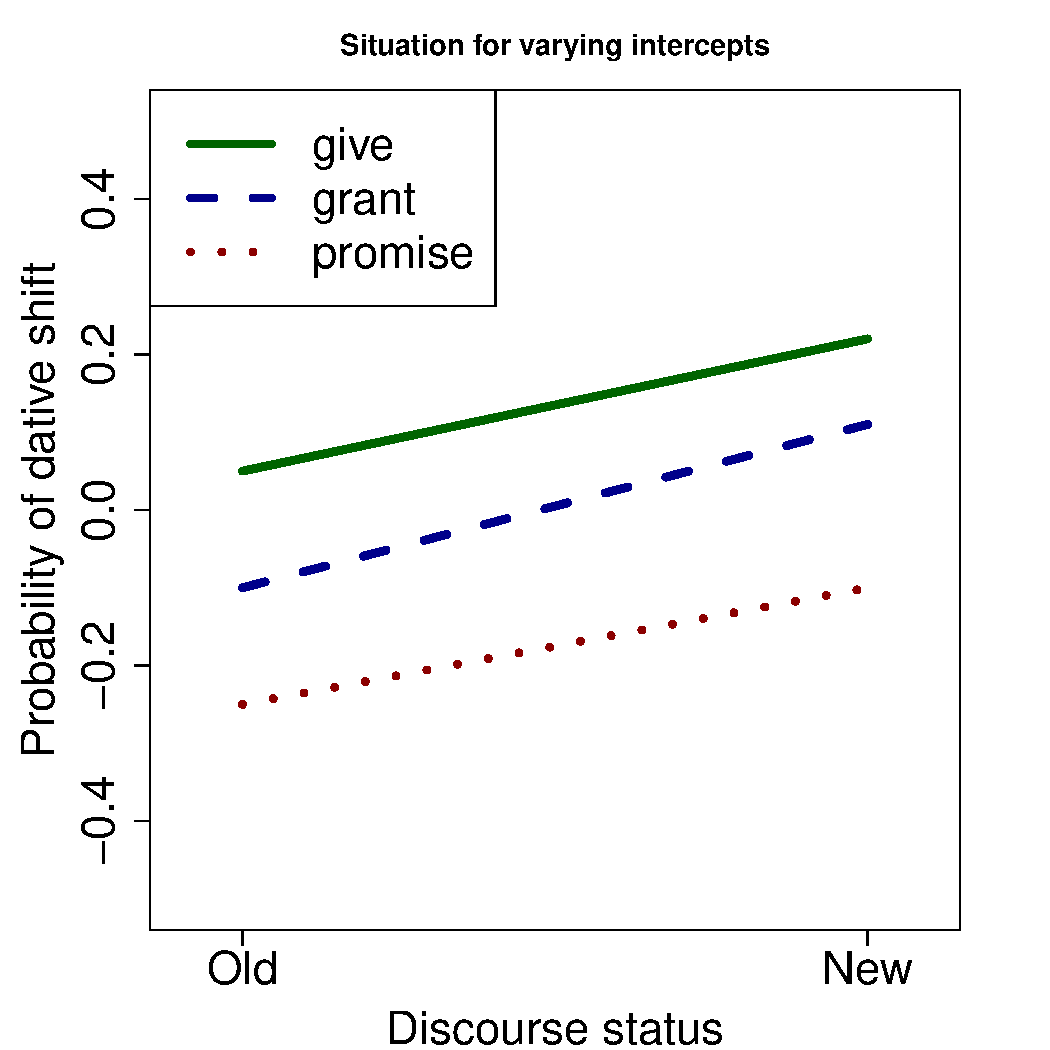
\includegraphics[width=0.5\textwidth]{graphics/var_int}~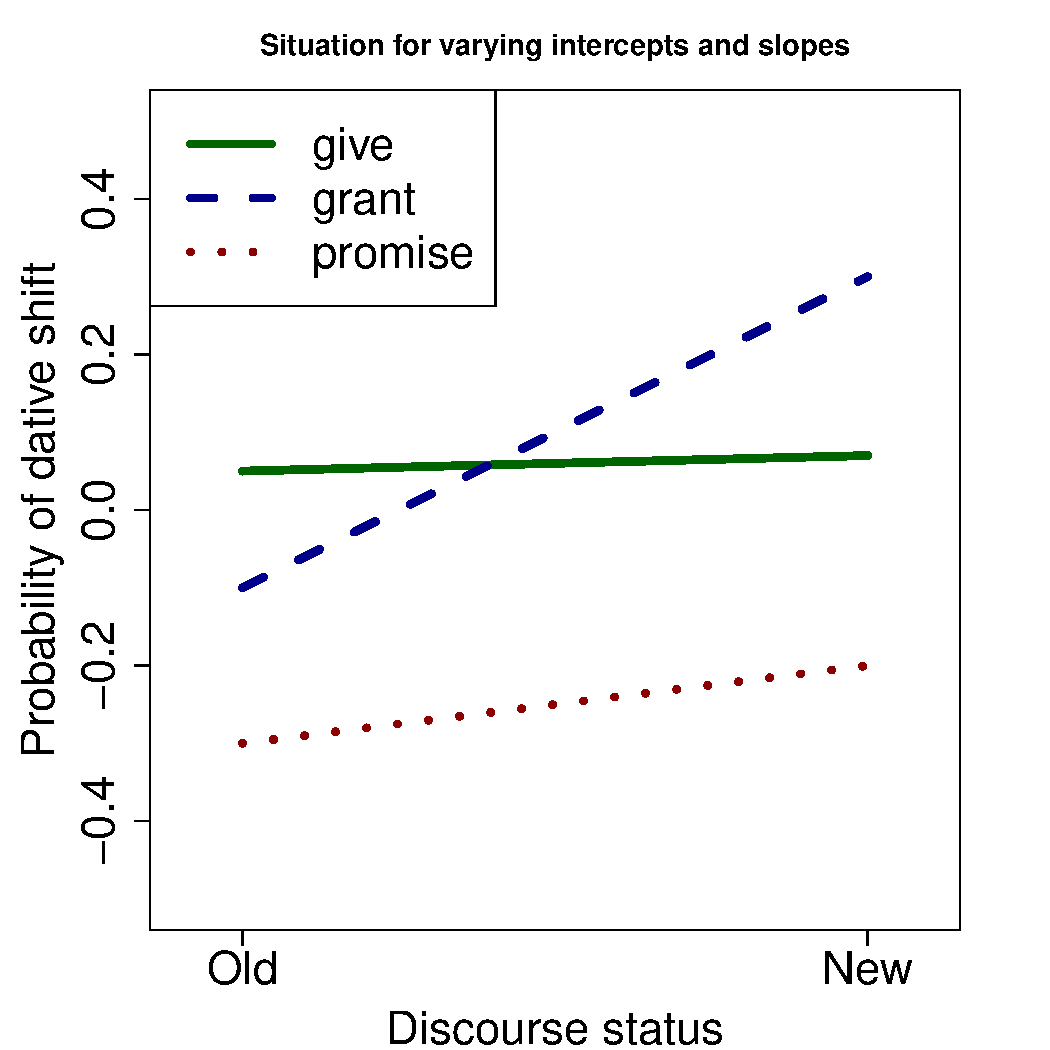
\includegraphics[width=0.5\textwidth]{graphics/var_int_slope}
  \caption{Illustration of data in situations for varying intercepts or varying intercepts and additional varying slopes}
  \label{fig:varintlsope}
\end{figure}

We assume that we are looking at an alternation phenomenon like the dative alternation, wherein we are interested in the probability that, under given circumstances, the dative shift construction is chosen.
When examining the data, it turns out that the probability of the dative shift changes for \textit{old} and \textit{new} dative NPs.
The verb lemma also influences the probability of either variant being used.
The situation can now be as in the left or the right panel of Figure~\ref{fig:varintlsope}.
In the left panel, the overall level in probability changes with the verb lemma, but for each verb lemma, the values change roughly accordingly in exemplars with old and new dative NPs.
Note that the lines are not perfectly parallel because the figure is supposed to be an illustration of a data set rather than a fitted model, and we always expect some chance variation in data sets.
In the right panel, however, the overall levels are different between lemmas, but the lemma-specific tendencies also vary between exemplars with old and new NPs.
This is actually nothing but an interaction between two factors (verb lemma and discourse status).
However, if the verb lemma factor is used as a random effect grouping factor, the interaction is modeled as a so-called \textit{random slope}.
In the next section, it is shown how all the different types of data sets discussed so far can be modeled using fixed effects models or, alternatively, using mixed effects.
Which one is more appropriate will be argued to be better understood as a technical rather than a conceptual question.


\subsection{Model specification and modeling assumptions}
\label{sec:modelspecificationandmodelingassumptions}

In this section, it is discussed how the specification of mixed models differs from that of fixed effects models, and that for each model with random effects there is an alternative models with only fixed effects.
It is based mostly on Part 2A of \citet{GelmanHill2006} (pp.~235--342).
% A major focus is on the question of when to use fixed and random effects.
% The amount of technicality and notation is kept at the absolute minimum, but a few notational conventions are introduced to enable readers to understand both the output of \texttt{lme4} and other packages in R as well as the literature on mixed models.
% To make successful practical use of mixed models, some level of fundamental understanding is required.

\subsubsection{Simple random intercepts}
\label{sec:simplerandomintercepts}

Readers with experience in fixed effects modeling should see that a grouping factor encoding the verb lemma and all the other grouping factors discussed in the previous sections could be specified as a normal fixed effect in a GLM.
In such a case, each of the $m$ levels of the speaker factor is dummy-coded, and for all but one of these binary dummy variables, a coefficient is estimated.
Logistic regression examples are used throughout this section, and we begin with the fictional corpus study of the dative alternation introduced in Sections~\ref{sec:hierarchicalormultilevelmodels} and \ref{sec:randominterceptsandslopes}.
We first specify a minimal model with only the dummies of the lemma grouping factor and one other (binary) predictor, namely discourse status.
There are $m$ verb lemmas (\ie groups) and $n$ observations.
As index variables, we use $j$ for groups and $i$ for observations.
In general, $\alpha$ is used for intercepts and $\beta$ for coefficients.
A specification of such a model is given in (\ref{eq:glm01}).

\begin{equation}
  Pr(y^i=1)=logit^{-1}(\alpha_0+\beta_d\cdot x_{d}^i+\beta_{l_1}\cdot x_{l_1}^i+\beta_{l_2}\cdot x_{l_2}^i+\cdots+\beta_{l_{m-1}}\cdot x_{l_{m-1}}^i)
  \label{eq:glm01}
\end{equation}

This models the estimate of the probability ($Pr$) that in observation $i$, the outcome variable $y^i$ is $1$, \ie that dative shift occurs.
$\alpha_0$ is the intercept, $\beta_d$ is the coefficient for the effect of discourse status.
$x_d^i$ is the value of the variable that encodes the discourse status for exemplar $i$ ($0$ for discourse-old NPs and $1$ for discourse-new NPs).
Furthermore, $\beta_{l_j}$ are the coefficients for the lemma dummy variables.
Finally, $x_{l_j}^i$ is the value ($0$ or $1$) for lemma $j$ in observation $i$.
If in exemplar $64$, the lemma is \textit{give} and \textit{give} is encoded as group $12$, then $i=64$, $j=12$, and $x_{l_{12}}^{64}=1$, whereas all $x_{l_j}^{64}=0$ with $j\neq12$.
Because one verb lemma dummy variable is on the intercept $\alpha_0$ and thus used as a reference, we only estimate $m-1$ instead of $m$ coefficients, \ie $j=1,\cdots,m-1$.%
\footnote{Picking one dummy as a reference level is necessary because otherwise infinitely many equivalent estimates of the model coefficients exist because one could simply add a constant to the intercept and subtract it from the dummies.
However, the estimator works under the assumption that there is a unique maximum likelihood estimate for the coefficient matrix.}
The function $logit^{-1}$ is the \textit{link function}, and its argument is the \textit{linear term} of the model.
It is obvious that in such a model, the effect of each verb lemma is treated as a fixed population parameter, exactly the same as the effect of discourse status.
% The coefficient $\beta_d$ is estimated in exactly the same way as each $\beta_{l_j}$.

If we treat the same grouping factor as a random intercept, we let the intercept vary by group, and we give the varying intercepts a distribution instead of estimating $m-1$ coefficients.
This is the relevant difference between a fixed effect and a random effect.
The model specification then looks like in (\ref{eq:glmm01}).

\begin{equation}
  P(y^i=1)=logit^{-1}(\alpha_{l}^{j[i]}+\beta_d\cdot x_d^i)
  \label{eq:glmm01}
\end{equation}

We now have an intercept $\alpha_l^{j[i]}$ which varies by group (instead of one term with its own coefficient per group).
We use the notation $\alpha_l^{j[i]}$ (borrowed in a modified form from \citealt{GelmanHill2006}) to indicate that the correct $j$-th lemma intercept is chosen for the $i$-th observation.
For example, if in exemplar $64$, the lemma is \textit{give}, which is group $12$, then $i=64$ and $j[64]=12$ (\ie the group appropriate for exemplar $64$ is group $12$), and $\alpha_l^{j[64]}=\alpha_l^{12}$.
The term $\beta_d\cdot x_d^i$ for the effect of discourse status remains unchanged when going from (\ref{eq:glm01}) to (\ref{eq:glmm01}).
Crucially, instead of estimating a batch of coefficients for the lemma effect, $\alpha_l$ is itself modeled, and random terms are predicted for each level of the grouping factor.
For this, the assumption in (\ref{eq:glmm02}) is made.

\begin{equation}
  \alpha_l^j\sim N(\mu_l,\sigma_l^2)
  \label{eq:glmm02}
\end{equation}

This is standard notation to indicate that the values of $\alpha_l^j$ follow a normal distribution with mean $\mu_l$ and a variance of $\sigma_l^2$.
In fact, we can regard (\ref{eq:glmm02}) as a minimal second-level model already, although one which simply predicts varying intercepts from a normal distribution.
All more complex models to be discussed below are extensions of this approach.
In the next section, the consequences of going from a fixed effect to a random effect are discussed.

\subsubsection{Choosing between random and fixed effects}
\label{sec:choosingbetweenrandomandfixedeffects}

There are primarily two points to consider which influence the decision to use random effects.
First, the variance in the intercepts (and for random intercept-random slope models also the covariance between intercepts and slopes) needs to be estimated.
Second, the random intercepts can be understood as a compromise between fitting separate models for each group of the grouping factor (\textit{no pooling}) and fitting a model while ignoring the grouping factor altogether (\textit{complete pooling}), see \citet[Ch.~12]{GelmanHill2006}.
% While all conditions which were discussed in the previous chapter (independence of observations, non-collinearity, etc.) must also be met by hierarchical models, these two points add additional conditions.

As was stated above in (\ref{eq:glmm02}), the random intercepts are assumed to follow a normal distribution, and the variance $\sigma_l^2$ needs to be estimated with sufficient precision.
From the estimated variance and the data, the estimator then predicts the \textit{conditional modes} in GLMMs (\textit{conditional means} in LMMs) for each group (see \citealt[Ch.~1]{Bates2010}), which is the numerical value which software packages like \texttt{lme4} produce for each level of the grouping factor.
% , and these values are sometimes sloppily called ``random effects'' by practitioners.
This procedure, however, requires that the number of groups must not be too low to effectively achieve this.
As a rule of thumb, fewer than five levels means that a grouping factor should be included as a fixed effect, regardless of its conceptual nature.
Even if there is a default recommendation to use a speaker grouping variable as a random effect, it is ill-advised to do so if there are exemplars from less than five speakers in the sample.
% Very often, the estimator will fail anyway under such conditions.
% Thus, a random effect might be the best option for technical reasons.

If, however, the number of groups is reasonably large, the next thing to consider is the number of observations per group.
Alternatives to using a random effect would be to estimate a separate model for each level of the grouping factor, or to include it as a fixed effect.
In both cases the effects are not treated as random variables, and fixed coefficients per group are estimated without taking the between-group variance into account.
% The estimation of coefficients for a (dummy-coded) fixed effect becomes less precise and feasible with large numbers of levels or when there are levels with very few observations.
With a random effect, however, the conditional modes\slash means are pulled (\textit{shrunken}) towards the overall intercept (\textit{shrinkage}).
When there the number of observations in a group is low, the conditional mode\slash mean is simply shrunken more strongly, predicting only a small deviation from the overall tendency.
Fixed effect estimates, on the other hand, become inexact and will probably be dismissed because of growing uncertainty in the estimate (large confidence intervals, non-significance) when the number of observations in a levels is low.
Put differently, low numbers of observations in all or some groups are often detrimental for using fixed effects grouping factors.
Random effects can deal with situations like this much better because of shrinkage.
On the downside, a strongly shrunken conditional mode cannot be distinguished straightforwardly from a conditional mode of a group which simply does not deviate a lot from the mean.
For fixed effects, we have both the estimate and the significance test, but for random effects, we only have the prediction of the conditional mode\slash mean.
Thus, including a grouping factor as a random effect might be the only way of using it at all when the estimation as a fixed effect fails.

This section closes with an illustration.%
\footnote{The code for these and other simulations is available under a Creative Commons Attribution license: \url{https://github.com/rsling/Rstuff/tree/master/simulations/glmm}}
For this, 1,000 data sets were simulated which corresponded to the model in (\ref{eq:glmm03}) and (\ref{eq:glmm04}).
We drop the subscripts on $\alpha$, $\beta$, and $\mu$ for convenience since there is only one random intercept.

\begin{align}
  P(y^i=1) & =logit^{-1}(\alpha^{j[i]}+\beta_1\cdot x_1^i+\beta_2^i\cdot x_2^i)
  \label{eq:glmm03}\\
  \alpha^j & \sim N(\mu, \sigma)\label{eq:glmm04}
\end{align}

Again, this could be a model of a binary alternation.
$x_1$ is a binary variable (such as given\slash new) and $x_2$ a continuous variable (such as NP length).
Since the data were simulated, the parameters to be estimated were known: $\beta_1=0.8$, $\beta_2=-1.3$, $\mu=0$, $\sigma=1.5$.
The number of groups was set to $5$, the simulated values of the grouping factor were identical in each simulation, and there were $20$ observations per group.
Figure~\ref{fig:glmmj5i20} shows the distribution of the group levels based on the conditional modes predicted of all but the first group in the $1,000$ simulations.
Figure~\ref{fig:glmj5i20} shows the group estimates from a model where the grouping factor was added as a fixed effect.%
\footnote{The plots do not show the distribution of the raw conditional modes and coefficient estimates of the fixed effects.
Rather, the overall intercept was taken into account, and the plots thus show the distribution of the per-group prediction of the models, all other things being equal.
This is what was pre-specified in the simulations.}

\begin{figure}[!htpb]
  \centering
  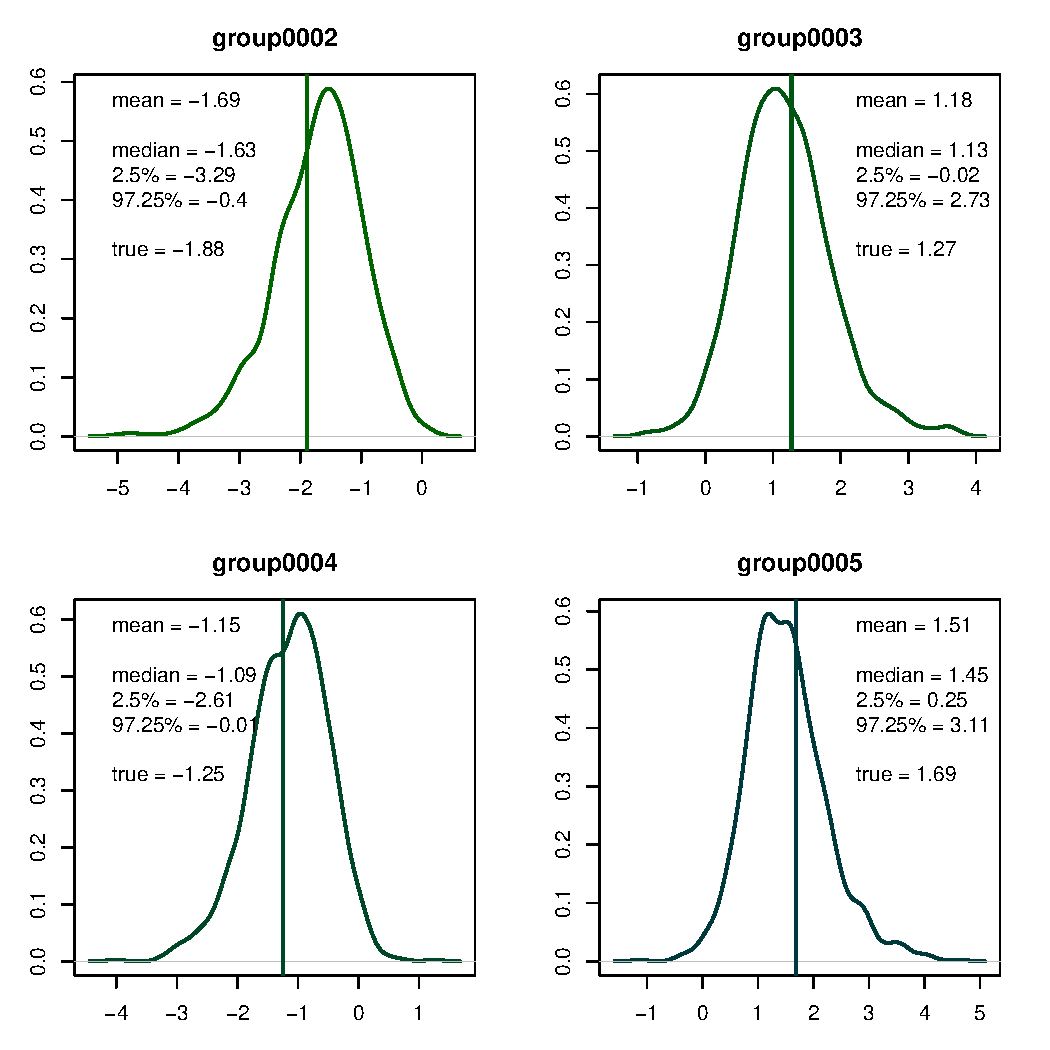
\includegraphics[width=0.6\textwidth]{graphics/glmmj5i20}
  \caption{Group levels in sample GLMM based on predicted random effect (conditional mode); 5 groups; 20 observations per group; 1,000 simulations; the horizontal line marks the true value}
  \label{fig:glmmj5i20}
\end{figure}
\begin{figure}[!htpb]
  \centering
  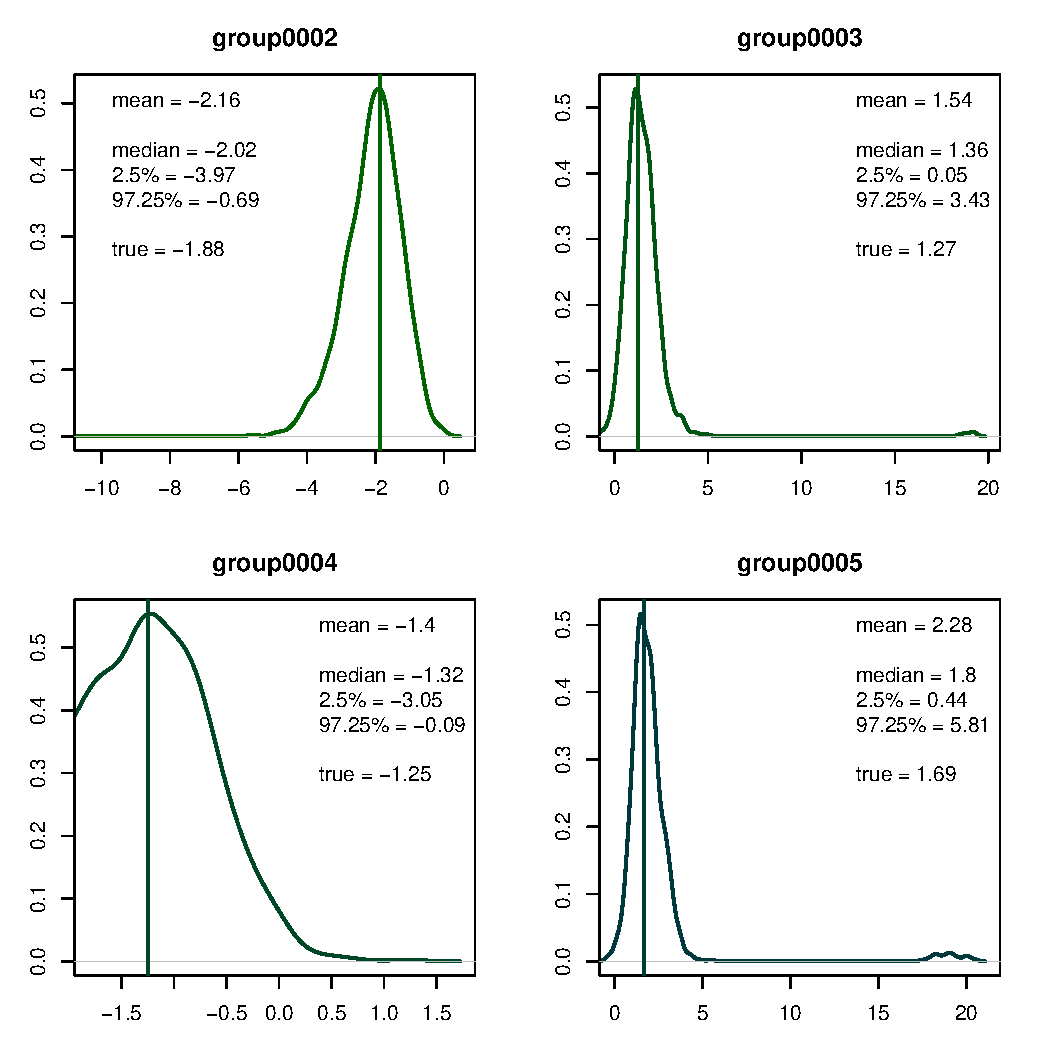
\includegraphics[width=0.6\textwidth]{graphics/glmj5i20}
  \caption{Estimated fixed effects for the grouping factor in sample GLM; 5 groups; 20 observations per level of the grouping factor; 1,000 simulations; the horizontal line marks the true value}
  \label{fig:glmj5i20}
\end{figure}

The per-group predictions lean slightly towards $0$ in the GLMM (Figure~\ref{fig:glmmj5i20}), but the fixed effects estimates in the GLM are prone to occasional misestimations.
While the overall spread is roughly the same for both approaches, the GLM estimates have massive outliers (down to approximately $-10$ and up to $20$), which leads to slightly larger 95\% intervals.
Even with as few as five levels of a grouping factor, however, random and fixed effects lead to very similar results, albeit with different advantages and disadvantages.
A few more differences will be discussed in Sections~\ref{sec:significancetestingandcoefficientsofdetermination} and \ref{sec:morecomplexmodels}.


\subsubsection{Significance testing, model selection and coefficients of determination}
\label{sec:significancetestingandcoefficientsofdetermination}

One commonly given reason to use a random effect is that ``the researchers are not interested in the individual levels of the random effect factor'' (or variations thereof).
Such recommendations should be taken with a grain of salt.
\citet[245--247]{GelmanHill2006} summarise the diverging and partially contradicting recommendations for what should be a random effect along with their motivations.
They conclude that there is essentially no clean conceptual or mathematical way of deciding what should be a random effect and what a fixed effect.
In this chapter, a more technical approach was therefore suggested.

However, it is not adequate to do any kind of significance test on the levels of the random effect because they are not estimates in the technical sense.
% The conditional modes are not estimates, and only for estimates is significance testing a well-defined activity.
There are ways of calculating confidence intervals for conditional modes (see Section~\ref{sec:specifyingmodelsusinglme4inr}), but they should not be misused for talking about significance.
% If this is absolutely required, fixed effects are the way to go.
Not doing significance tests for single levels of the grouping factor does, however, not mean that the researcher is not interested in the individual conditional modes, which is proven by the fact that they are often reproduced in research papers, for example in the form of a dot plot.
Also, the simulation in Section~\ref{sec:choosingbetweenrandomandfixedeffects} shows that we can use a random effect and still get a good idea of the per-group tendencies.
Additionally, a random effect allows the researcher to quantify the between-group variance, which is not possible in the same way with fixed effects.

A related question is \textit{model selection}, \ie whether the inclusion of the random effect improves the model quality.
It is recommended here to include all conceptually necessary random effects and only remove them if they have no effect.
To check this, the estimated between-group variance is the first thing to look at.
If it is close to $0$, there is most likely not much going on between groups, or there simply was not enough data to estimate the variance.
In LMMs, it is possible to compare the residual (observation-level) variance with the between-group variance to see which one is larger, and to which degree.
If, for example, the residual variance is $\sigma_{\epsilon}=0.2$ and the between-group variance is $\sigma_{\alpha}=0.8$, then we can say that the between-group variance is four times larger than the residual variance, which would indicate a high importance of the random effect.
This comparison is impossible in GLMMs because their (several types of) residuals do not have the same straightforward interpretation as in LMMs.
Furthermore, likelihood ratio (LR) tests are available for comparing a model including the random effect and a model not including it.
Such pairs of models, where one is strictly a simplification of the other, are called \textit{nested models} (not to be confused with \textit{nested effects} discussed in Section~\ref{sec:crossedandnestedeffects}).
An alternative option are parametric bootstrap replacements for the LR test.
%(see Section~\ref{sec:specifyingmodelsusinglme4inr}).
It is not appropriate to compare a GLMM with a random effect and a GLM with the same factor as a fixed effect using any test or metric (including information criteria).

Coefficients of determination (pseudo-$R^2$) can be used to give some idea of the model fit.
%should not be used for model selection, because they usually do not penalize complexity enough (\ie the pseudo-$R^2$ measures rise with added complexity).
%They can still be used to give some idea of the model fit, however.
For GLMMs, \citet{NakagawaSchielzeth2013} have proposed a method that distinguishes between \textit{marginal} $R^2$ (fixed-effects-only) and \textit{conditional} $R^2$ (including random effects).
This has become a de facto standard, and we now show its consistency with Nagelkerke's $R^2$ for GLMs.
Using the simulations described in the last section, Figures~\ref{fig:rsqglmmj5i20} and \ref{fig:rsqglmj5i20} show that the marginal $R^2$ is roughly the same as Nagelkerke's $R^2$ in a GLM which ignores the grouping factor, and the conditional $R^2$ is roughly the same as Nagelkerke's $R^2$ in a GLM which includes the grouping factor as a fixed effect.
It should be noted that the simulations were explicitly designed such that the grouping factor (five levels with enough observations per level) could be used successfully as a fixed effect and a random effect, which is usually not the case with real data.

\begin{figure}[!htpb]
  \centering
  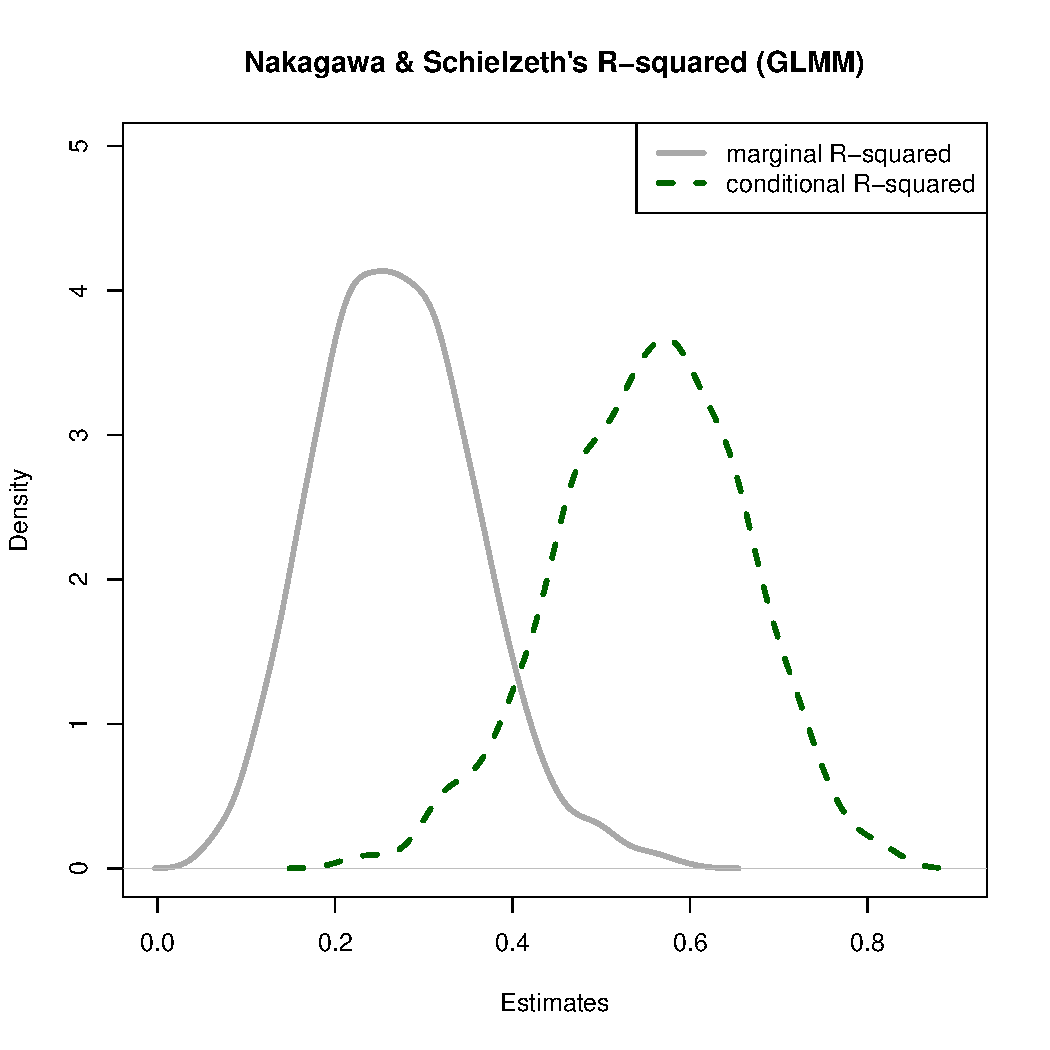
\includegraphics[width=0.6\textwidth]{graphics/rsqglmmj5i20}
  \caption{Distribution of Nakagawa \& Schielzeth's $R^2$ in the simulations described in Section~\ref{sec:choosingbetweenrandomandfixedeffects}}
  \label{fig:rsqglmmj5i20}
\end{figure}

\begin{figure}[!htpb]
  \centering
  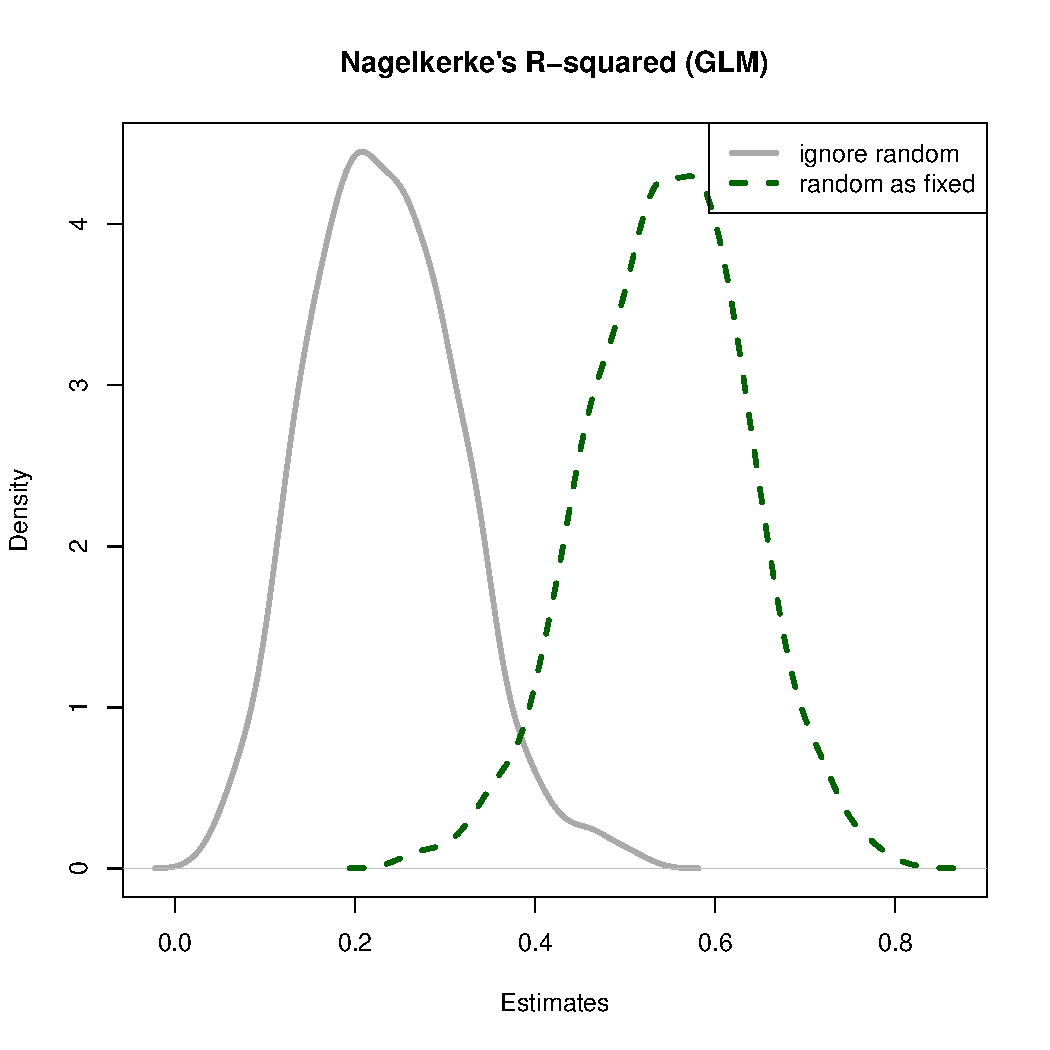
\includegraphics[width=0.6\textwidth]{graphics/rsqglmj5i20}
  \caption{Nagelkerke's $R^2$ in the simulations described in Section~\ref{sec:choosingbetweenrandomandfixedeffects} for a GLM that ignores the grouping factor and a model that includes it as a fixed effect}
  \label{fig:rsqglmj5i20}
\end{figure}

\subsubsection{More complex models}
\label{sec:morecomplexmodels}

% This section shows briefly how more complex models are specified before Section~\ref{sec:specifyingmodelsusinglme4inr} demonstrates how models are estimated in R, including interpretations of the output.

\paragraph{Varying intercepts and slopes}

While it is possible to have just a varying slope, this is rarely useful, and we discuss only varying-intercept and varying-slope (VIVS) models.
We extend the simple model from (\ref{eq:glmm01}), and the fixed effect coefficients for which a random slope is specified simply receive group indices; see (\ref{eq:glmm05}).
Put simply, instead of a fixed coefficient, coefficients are predicted and assumed to come from a random (normal) distribution.
We use $\beta_{d:l}$ to denote the coefficient for discourse status varying by lemma.

\begin{equation}
  P(y^i=1)=logit^{-1}(\alpha_{l}^{j[i]}+\beta_{d:l}^{j[i]}\cdot x_d^i)
  \label{eq:glmm05}
\end{equation}

A source of problems in VIVS models is the fact that in addition to the variance in the intercepts and slopes, the covariance between them has to be estimated.
If in groups with a higher-than-average intercept, the slope is also higher than average, they are positively correlated, and vice versa.
These relations are captured in the covariance.
Therefore, condition (\ref{eq:glmm06}) is added, where the indices $l$ and $d:l$ are omitted for readability.

\begin{equation} 
  \left( \begin{smallmatrix} \alpha^j \\ \beta^j \end{smallmatrix}\right) \sim
    \left(
    \left( \begin{smallmatrix} \mu_{\alpha}\vphantom{\beta^j} \\ \mu_{\beta}\vphantom{\beta^j} \end{smallmatrix} \right), 
      \left( \begin{smallmatrix} \sigma_{\alpha}^2 & \rho\sigma_{\alpha}\sigma_{\beta} \\
	\rho\sigma_{\alpha}\sigma_{\beta} & \sigma_{\beta}^2 \end{smallmatrix} \right)
    \right)
  \label{eq:glmm06}
\end{equation}

(\ref{eq:glmm06}) says that the joint distribution of the intercepts $\alpha^j$ and the slopes $\beta^j$ follows a bivariate normal distribution with means $\mu_{\alpha}$ and $\mu_{\beta}$.
The variance in the intercepts is $\sigma_{\alpha}$, the variance in the slopes is $\sigma_{\beta}$, and the coefficient for the covariance between them is $\rho$.
Figure~\ref{fig:multnorm} shows the bivariate density distributions for two (1) negatively correlated, (2) non-correlated, and (3) positively correlated normally distributed variables.

\begin{figure}[!htpb]
  \centering
  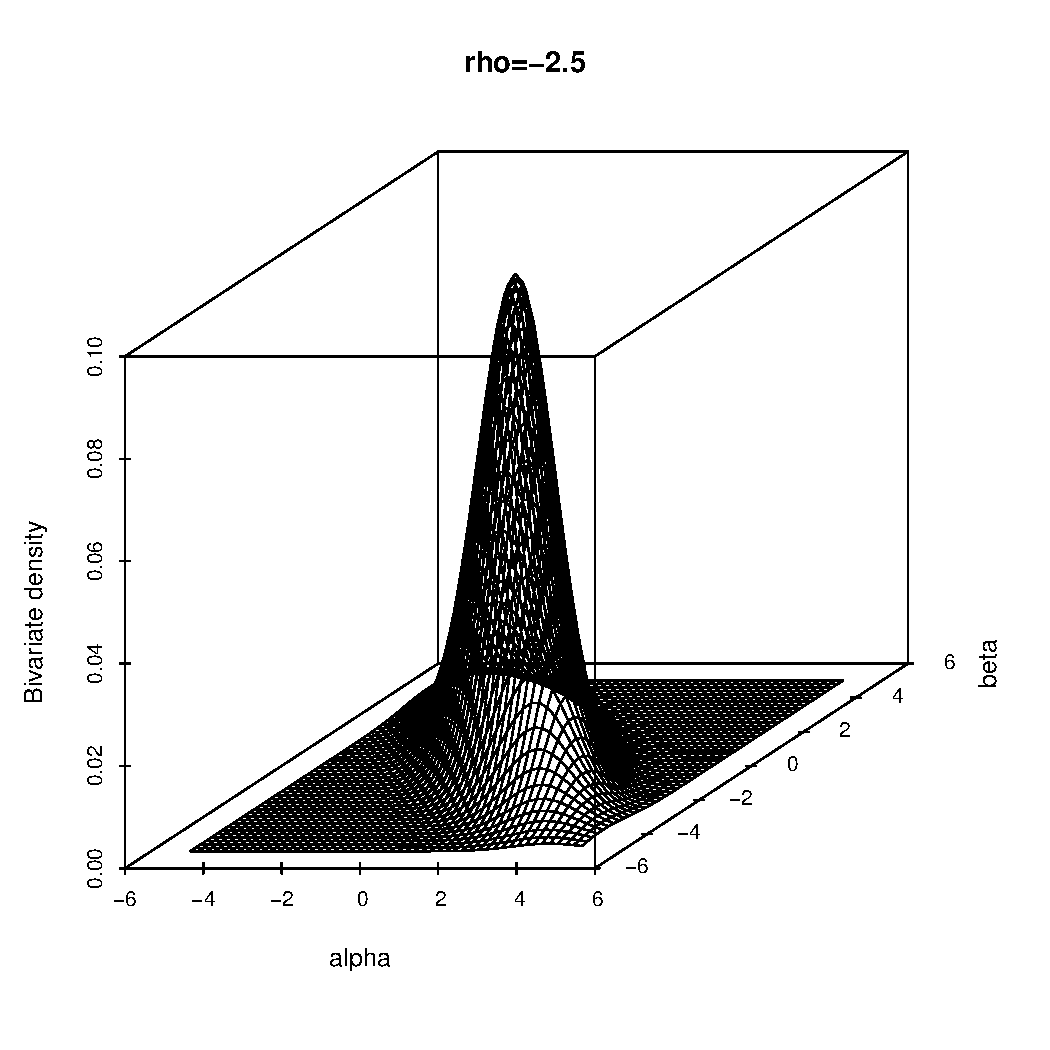
\includegraphics[width=0.33\textwidth]{graphics/multnorm1}~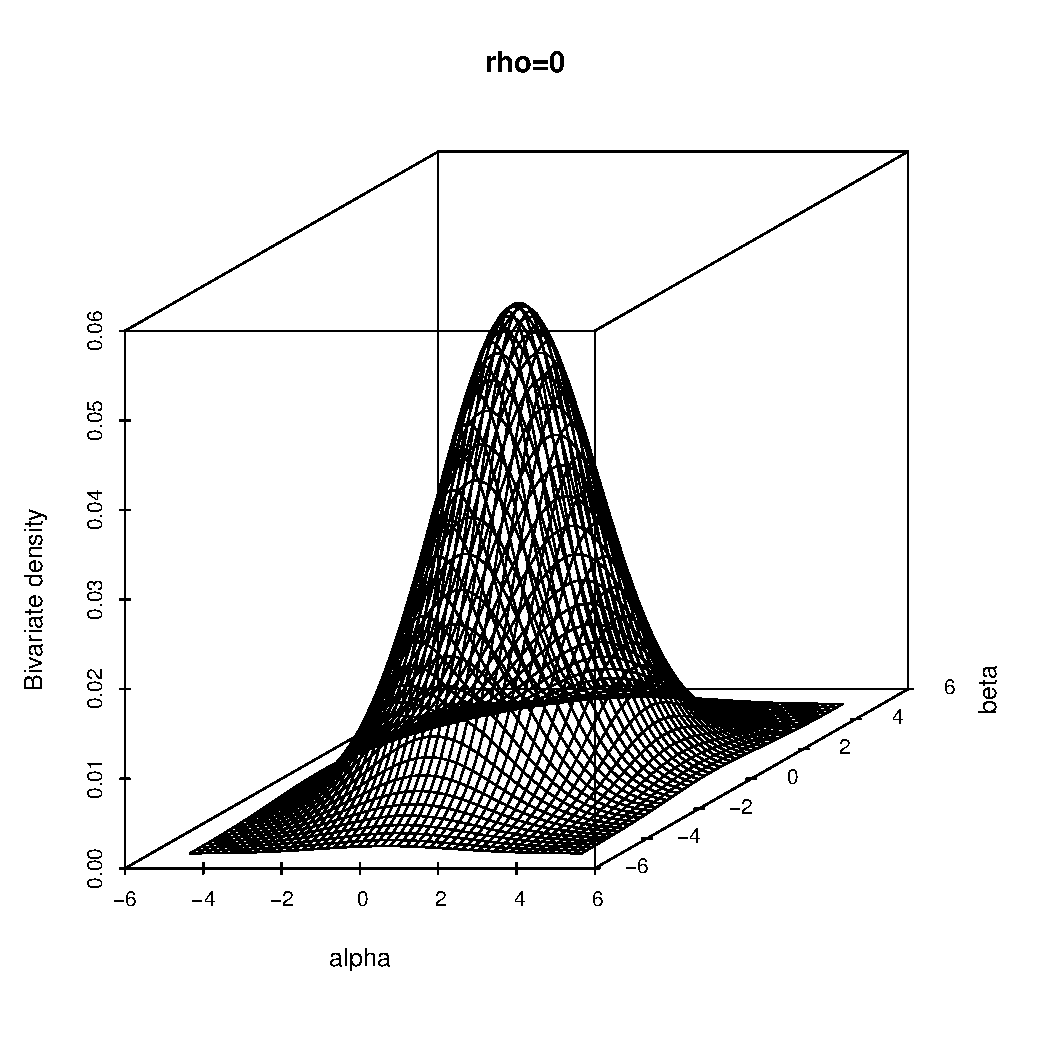
\includegraphics[width=0.33\textwidth]{graphics/multnorm2}~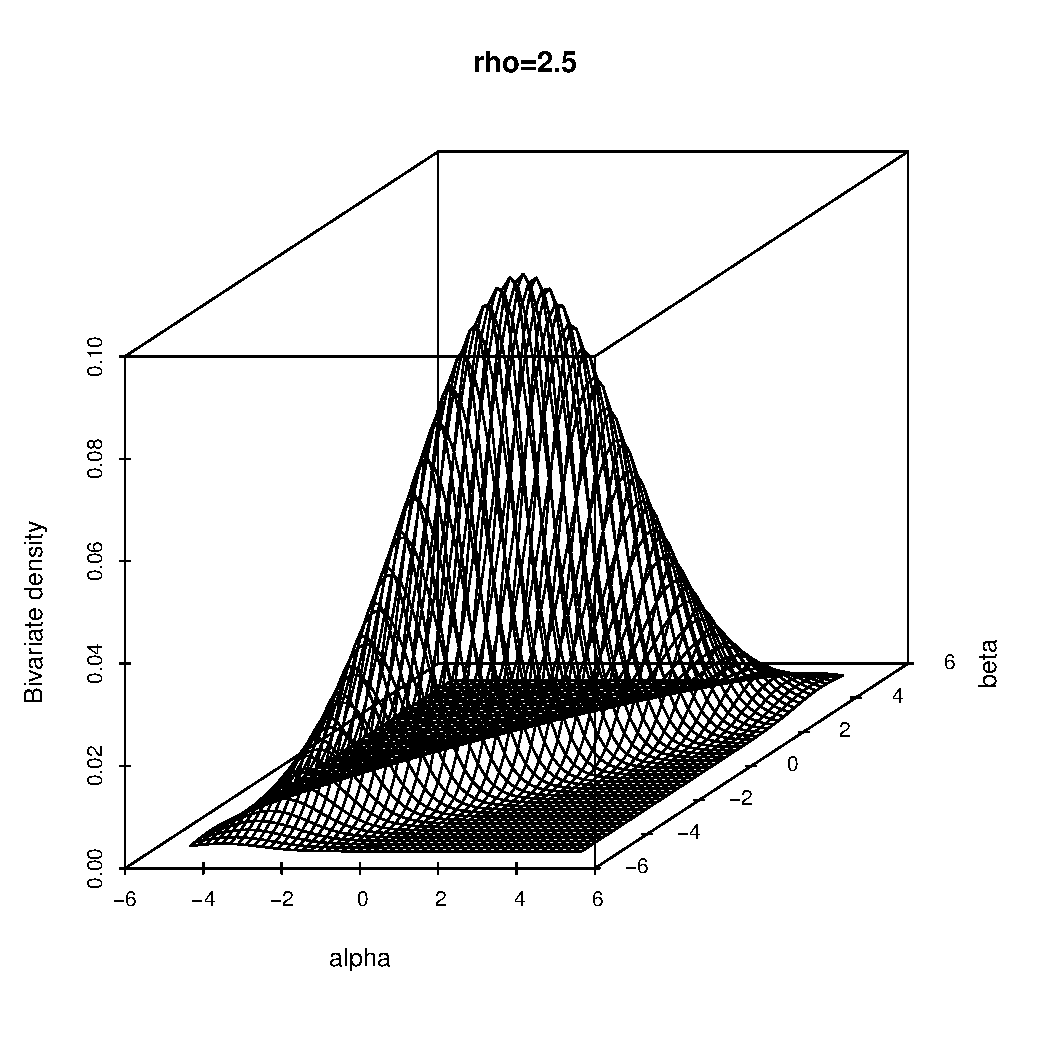
\includegraphics[width=0.33\textwidth]{graphics/multnorm3}
  \caption{Bivariate normal density distribution with different correlation strengths ($\rho$); $\sigma_{\alpha}=\sigma_{\beta}=3$; $\mu_{\alpha}=\mu_{\beta}=0$}
  \label{fig:multnorm}
\end{figure}

The number of variance parameters to be estimated obviously increases with more complex model specifications, and the estimation of the parameters in the presence of complex variance-covariance matrices requires considerably more data than estimating a single variance parameter.
The estimator might converge, but typically covariance estimates of $-1$ or $1$ indicate that the data was too sparse for a successful estimation of the parameter.
In this case, the model is \textit{over-parametrized} and needs to be simplified.
% In Section~\ref{sec:afterfittingmodelswithlme4}, it will be shown how to interpret the \texttt{lme4} output appropriately.

\paragraph{Nested and crossed random effects}

As it was explained in Section~\ref{sec:crossedandnestedeffects}, nested random effects are adequate when grouping factors are nested within other grouping factors.
Technically, while varying slopes can be understood as interactions between a fixed and a random effect, nested random intercepts can be understood interactions between two or more random effects.
Crossed random effects are just several unrelated random effects.
(\ref{eq:glmm07}) shows the model specification, extending (\ref{eq:glmm01}) with a varying intercept $\alpha_s$.
This could be for example semantic classes which nest individual lemmas.
It could also be another grouping factor for speaker, completely unrelated to the lemmas.

\begin{equation}
  P(y^i=1)=logit^{-1}(\alpha_{s}^{k[i]}+\alpha_{l}^{j[i]}+\beta_d\cdot x_d^i)
  \label{eq:glmm07}
\end{equation}

The difference is that in the nested case, $k[i]=k[j]$, \ie the level of the nesting factor can be selected based on the nested factor as well as based on the single observation.
As was mentioned in Section~\ref{sec:crossedandnestedeffects}, the questions is rather one of how the way the data are organised.
% In the model specification, there are no obvious differences.

\paragraph{Second-level predictors}

In Section~\ref{sec:hierarchicalormultilevelmodels}, situations were introduced where the random effects themselves can be partially predicted from fixed-effects.
In this case, an additional linear model is specified for the random effect instead of the simple normal distribution predictor.
We extend (\ref{eq:glmm01}) by a predictor $\gamma_f$ for the lemma frequency.
The lemma frequencies themselves, we denote by $u_f$, and we index them with $j$, just like the verb lemmas.
This is reasonable because for each verb lemma, there is exactly one frequency.
The first-level model specification remains the same, namely (\ref{eq:glmm08}).

\begin{equation}
  P(y^i=1)=logit^{-1}(\alpha_{l}^{j[i]}+\beta_d\cdot x_d^i)
  \label{eq:glmm08}
\end{equation}

However, instead of (\ref{eq:glmm02}), the varying intercept is predicted from (\ref{eq:glmm09}).

\begin{equation}
  \alpha_l^j\sim N(\gamma_0+\gamma_f\cdot u_f^j,\sigma_l^2)
  \label{eq:glmm09}
\end{equation}

Instead of just the mean of the $\alpha_j$ values, the model in (\ref{eq:glmm09}) specifies a second-level intercept $\gamma_0$ and a second-level fixed coefficient $\gamma_f$.
% If the lemma frequency plays a role, this approach can lead to a more precise prediction of the varying first-level intercept compared to the less elaborate approach in (\ref{eq:glmm02}).
% True multilevel models increase the complexity of GLMMs, especially if third-level models, fourth-level models, etc. are used.
% Situations for multilevel modeling are quite frequently encountered, however.
% Especially when it comes to speakers as random effects, the age, the gender, the region of birth (if this grouping factor has too few levels to be used as a random effect nesting speakers), etc.\ are ideal second-level predictors.
% The \texttt{lme4} syntax treats second-level predictors like interactions between a fixed and a random effect, see also Section~\ref{sec:specifyingmodelsusinglme4inr}.

% Readers finding it difficult to see why (\ref{eq:glmm09}) is a plain linear model could consider the equivalent formulation in (\ref{eq:glmm10}) and (\ref{eq:glmm11}).
%  
% \begin{align}
%   \alpha_l^j   =    & \gamma_0+\gamma_f\cdot u_j^j+\epsilon_l^j \label{eq:glmm10}\\
%   \epsilon_l^j \sim & N(0, \sigma^2) \label{eq:glmm11}
% \end{align}

\paragraph{Remarks on models for longitudinal studies}

A longitudinal study is one wherein single subjects (usually speakers) are observed at different points in time, for example second-language learners after different years of learning a second language.
% This section briefly discusses the main points to consider when such models -- which can get quite complex -- are specified.
First, the observations are obviously grouped by the individual speakers.
It is thus recommended to include the speaker grouping factor, typically as a random effect.
% either as a fixed effect (up to five speakers) or random effect (more speakers).
Second, there might be time parameters such as years of learning.
% Third, the errors might be correlated.

We now assume we have a (fictional) sample from a learner corpus of German as a second language.
In a logistic regression, we examine whether Swedish and English learners use the weak or the strong forms of attributive adjectives in NPs with a determiner.
Grammatically, the crucial variable is whether the determiner has itself a strong ending or not, and we include an appropriate first-level term $\beta_d\cdot x_d^i$ in the model.
A random effect for individual learners is also included as $\alpha_l^{j[i]}$.
Additionally, we add a term for the number of years the learners have learned German.
% (potentially logarithmized or otherwise transformed).
However, since learners progress with different speed, a random slope is indicated, and the term becomes $\beta_{y:l}^{j[i]}\cdot x_y^i$.
The first-level model is thus (\ref{eq:glmm013}).

\begin{equation}
  P(y^i=1)=logit^{-1}(\alpha_l^{j[i]} + \beta_d\cdot x_d^i + \beta_{y:l}^{j[i]}\cdot x_y^i)
  \label{eq:glmm013}
\end{equation}

The main purpose of our study might be to find out whether Swedish and English learners differ with respect to the phenomenon at hand.
Therefore, the first language is added as a second-level predictor with the term $\gamma_f\cdot u_f^j$, where $u_f^j$ is $1$ if the language of learner $j$ is Swedish, and $0$ if it is English.
Since we have a random intercept and a random slope we need to distinguish between $\gamma_f^{\alpha}\cdot u_f^j$ for the random intercept and $\gamma_f^{\beta}\cdot u_f^j$ for the random slope.
The second level model to go with (\ref{eq:glmm013}) is (\ref{eq:glmm14}).

\begin{equation} 
  \left( \begin{smallmatrix} \alpha^j \\ \beta^j \end{smallmatrix}\right) \sim
    \left(
    \left( \begin{smallmatrix} \gamma_0^{\alpha}+\gamma_f^{\alpha}\cdot u_f^j \\ \gamma_0^{\beta}+\gamma_f^{\beta}\cdot u_f^j    \end{smallmatrix} \right), 
      \left( \begin{smallmatrix} \sigma_{\alpha}^2 & \rho\sigma_{\alpha}\sigma_{\beta} \\
	\rho\sigma_{\alpha}\sigma_{\beta} & \sigma_{\beta}^2 \end{smallmatrix} \right)
    \right)
  \label{eq:glmm14}
\end{equation}

Although this is a quite complex model already, there might be more problems.
The performance of learners after $n+1$ years of learning is usually correlated to a high degree with their performance after $n$ years.
This can lead to \textit{autocorrelation} in the errors, violating basic modeling assumptions.
To take care of this, model which allow for explicitly specified error structures must be used.
Anyone wishing to use such models will should consult further references (\eg \citealt{Fox2016} and \citealt{ZuurEa2009}).

\subsection{Specifying model using \texttt{lme4} in R}
\label{sec:specifyingmodelsusinglme4inr}

This section and the next focus on \texttt{lme4}, the standard package to do multilevel modeling in R with maximum likelihood methods \citep{BatesEa2015}.

\paragraph{Varying intercepts}

The functions \texttt{lmer} and \texttt{glmer} extend the syntax of \texttt{lm} and \texttt{glm}.
The varying intercept model in (\ref{eq:glmm01}) is specified as follows in R (using informative variable names instead of Greek letters).

\vspace{0.5\baselineskip}

\begin{lstlisting}
glmer(formula = construction ~ discourse + (1 | lemma),
      family = binominal(link=logit), data = my.data)
\end{lstlisting}

The pipe operator \texttt{x1|x2} can be read as \textit{x1 varies by x2}.
The intercept is denoted by \texttt{1}, and hence \texttt{(1|lemma)} simply says that the intercept varies by lemma.

\paragraph{Varying intercepts and slopes}

The VIVS model in (\ref{eq:glmm05}) is specified as follows (only the formula).

\vspace{0.5\baselineskip}

\begin{lstlisting}
construction ~ discourse + (1 + discourse | lemma)
\end{lstlisting}

Before the pipe, the part of the model is repeated that should be modeled as varying by the grouping factor after the pipe.
If a varying slope is specified, a varying intercept is silently assumed.
The last formula can therefore be abbreviated to the following equivalent one.

\vspace{0.5\baselineskip}

\begin{lstlisting}
construction ~ discourse + (discourse | lemma)
\end{lstlisting}

In order to let \textit{only} the slope vary, the intercept has to be removed explicitly from the random part of the formula.

\vspace{0.5\baselineskip}

\begin{lstlisting}
construction ~ discourse + (discourse - 1 | lemma)
\end{lstlisting}

\paragraph{Multiple random effects}

When there is more than one random effect, several bracketed terms are added.
The following is the recommended specification for models like (\ref{eq:glmm07}), regardless of whether the effects are nested or crossed.

\vspace{0.5\baselineskip}

\begin{lstlisting}
construction ~ discourse + (1 + | lemma) +
               (1 | semantics)
\end{lstlisting}

Sometimes the following notation is used for nested random effects, where \texttt{semantics} nests \texttt{lemma}.

\vspace{0.5\baselineskip}

\begin{lstlisting}
construction ~ discourse + (1 | semantics / lemma)
\end{lstlisting}

\texttt{lme4} expands this to the following underlying syntax, which shows more clearly that nesting is handled as a kind of interaction.

\vspace{0.5\baselineskip}

\begin{lstlisting}
construction ~ discourse + (1 | semantics) +
               (1 | semantics : lemma)
\end{lstlisting}

There is a random intercept for \texttt{semantics} and one for each combination of \texttt{semantics} and \texttt{lemma}
While these notations are seemingly very explicit about the nesting structure, they are not necessary under normal circumstances.
If the grouping factor \texttt{lemma} is nested within \texttt{semantics} (see Table~\ref{tab:nested}), \texttt{lme4} automatically treats it as nested, and the results are exactly the same with all the three aforementioned notations.

However, the following specification is \textit{not} equivalent and leads to problematic results.

\vspace{0.5\baselineskip}

\begin{lstlisting}
construction ~ discourse + (1 | semantics) +
               (1 | lemma) +
               (1 | semantics : lemma)
\end{lstlisting}

This instructs \texttt{lme4} to estimate the variance of \texttt{lemma} not just restricted to specific permutations of the levels of \texttt{lemma} and \texttt{semantics} (\ie \texttt{semantics : lemma}), but also outside of these specific permutations.
In the nested case, there are no occurrences outside of these permutations, however, and the variance for \texttt{lemma} alone will be estimated close to $0$, while the variance estimate for \texttt{semantics : lemma} will be distorted.

\begin{table}
  \centering
  \begin{tabular}{lll}
    \toprule
    \textbf{Exemplar} & \textbf{Speaker}  & \textbf{Region}        \\
    \midrule
                    1 &           D      &         Tyneside       \\
                    2 &           D      &         Tyneside       \\
                    3 &           R      &         Tyneside       \\
                    4 &           R      &         Tyneside       \\
                    5 &           D      &         Greater London \\
                    6 &           D      &         Greater London \\
                    7 &           R      &         Greater London \\
                    8 &           R      &         Greater London \\
    \bottomrule
  \end{tabular}
  \caption{Illustration of nested factors, organized suboptimally}
  \label{tab:nestedwrong}
\end{table}

There is one situation where the explicit notation for nested factors is necessary.
This is when the data are stored in a suboptimal way.
The suboptimal version of Table~\ref{tab:nested} would look something like Table~\ref{tab:nestedwrong}.
Here, the speaker factor is encoded as the initial letter of the name only.
Hence, Daryl and Dale (coming from two different regions) cannot be distinguisehd from each other, and Riley and Reed cannot, either.
This leaves \texttt{lme4} no way of recognizing that the data structure is nested, and the user has to explicitly provide that information.
It would, of course, be better \textit{not} to organize data that way.

\paragraph{Second-level predictors}

(\ref{eq:glmm08}) and (\ref{eq:glmm09}) have the following \texttt{lme4} syntax.

\vspace{0.5\baselineskip}

\begin{lstlisting}
construction ~ discourse + frequency + (1 | lemma)
\end{lstlisting}

If the data is organized as shown in Table~\ref{tab:multilevel} -- \ie, with the second-level regressor not having any variance within the levels of the grouping factor --, \texttt{lme4} will detect this and treat \texttt{frequency} as a second-level effect.
% This should be kept in mind when interpreting the results of the estimation.
However, second-level predictors for random slopes are more tricky to specify (see \citealt[280-282]{GelmanHill2006}).
Assuming that the effect of discourse status varies with the lemma, which itself comes with a second-level model including frequency as a regressor, the specification looks as follows.

\vspace{0.5\baselineskip}

\begin{lstlisting}
construction ~ discourse + frequency +
               discourse : frequency +
	       (1 + discourse | lemma)
\end{lstlisting}

A second-level regressor on a varying slope is thus an interaction between a first-level and a second-level fixed effect.

\subsection{After fitting models with \texttt{lme4}}
\label{sec:afterfittingmodelswithlme4}

\paragraph{Basics and varying intercepts}

The output for GLMMs in \texttt{lme4} can be understood straightforwardly after what was said in Sections~\ref{sec:fundamentals}.
Here is a possible output of the \texttt{summary} function for a fit of model (\ref{eq:glmm01}) and (\ref{eq:glmm02}), repeated here as (\ref{eq:glmm01r}) and (\ref{eq:glmm02r}).
Simulated data was used.

\begin{align}
  P(y^i=1) & = logit^{-1}(\alpha_{l}^{j[i]}+\beta_d\cdot x_d^i)
  \label{eq:glmm01r} \\
  \alpha_l^j & \sim N(\mu_l,\sigma_l^2)
  \label{eq:glmm02r}
\end{align}

\vspace{0.5\baselineskip}

\begin{lstlisting}
Generalized linear mixed model fit by maximum likelihood 
 Family: binomial  ( logit )
Formula: construction ~ discourse + (1 | lemma)
   Data: observations

Random effects:
 Groups Name        Variance Std.Dev.
 lemma  (Intercept) 1.29     1.136   
Number of obs: 250, groups:  lemma, 5

Fixed effects:
            Estimate Std. Error z value Pr(>|z|)    
(Intercept)   0.7638     0.5513   1.385    0.166    
discourse1    1.5064     0.3626   4.154 3.26e-05 ***
\end{lstlisting}

Some clutter as well as information which we do not interpret here (AIC, BIC, and information about the residuals) have been removed.
In this output, the \texttt{(Intercept)} estimate ($0.7638$) is $\hat{\mu}_l$, and the \texttt{Variance} estimate for the \texttt{lemma} random intercept ($1.29$) is $\hat{\sigma}_l^2$.%
\footnote{In general, the notation $\hat{v}$ denotes an estimate of the variable $v$.}
The estimate for \texttt{discourse1} ($1.5064$) corresponds to $\hat{\beta}_d$.
Finally, we learn that there were five different lemmas and $250$ observations in total.

To see whether the random intercept has a considerable influence, we should first look at the variance estimate.
Here, it is larger than one, which would be surprising if there were nothing going on in terms of between-lemma variation.
It is possible to compute confidence intervals for the variance estimate using the \texttt{confint} function.
Assuming the original model was stored in \texttt{alternation}, the following two alternatives work.

\vspace{0.5\baselineskip}

\begin{lstlisting}
  confint(alternation, parm="theta_", method = "profile")
  confint(alternation, parm="theta_", method = "boot",
          nsim = 250)
\end{lstlisting}

The profile method uses LR tests and the bootstrap method uses a parametric bootstrap.
For this model (where the variance estimate was $1.29$ and the true value used to generate the data was $1.5$), the profile method gives $0.5808\dots2.6433$ and the bootstrap with $250$ simulations gives $3.9665\cdot10^{-6}\dots1.8023$ as the $95\%$ confidence interval.
Since the bootstrap (especially with smaller original sample sizes as in this case) typically tends to run into replications where the estimation of the variance fails and is thus returned as $0$, the bootstrap interval is skewed to the left, while the profile confidence interval frames the true value symmetrically.
The bootstrap is thus not always more robust or intrinsically better.

Although the authors of the \texttt{lme4} package advise against it, a significance test on the deviances of a simple GLM and a GLMM with an added single random effect can be performed with the \texttt{anova} function.

\vspace{0.5\baselineskip}

\begin{lstlisting}
alternation.null <- glm(construction ~ discourse,
                        data = observations,
			family = binomial(link=logit))
anova(alternation, alternation.null)
\end{lstlisting}

The GLMM must be the first argument to \texttt{anova}.
In this case, the output looks like this, indicating a significant effect, although the p-values should not be considered highly reliable.

\vspace{0.5\baselineskip}

\begin{lstlisting}
Data: observations
Models:
null.model: construction ~ discourse
full.model: construction ~ discourse + (1 | lemma)
          Df  logLik deviance  Chisq Chi Df Pr(>Chisq)    
null.model 2 -134.52   269.05                             
full.model 3 -119.12   238.24 30.801      1  2.859e-08 ***
\end{lstlisting}

If the nested (simpler) model still contains a random effect, the \texttt{update} function can be used to build the simpler model.
Also, in addition to the \texttt{anova} command, there is a drop-in replacement for LR tests using bootstrap methods in the \texttt{pbkrtest} package \citep{HalekohHojsgaard2014}.

\vspace{0.5\baselineskip}

\begin{lstlisting}
alternation.1 <- glmer(construction ~ discourse +
                       (1 + | lemma) + (1 | semantics),
	               family = binominal(link=logit),
		       data = my.data)
alternation.2 <- update(object = alternation,
                        formula = construction ~
			          discourse +
                                  (1 + | lemma))

require(pbkrtest)
PBmodcomp(alternation.1, alternation.2, nsim = 250)
\end{lstlisting}

The coefficient of determination (pseudo-$R^2$) according to \citet{NakagawaSchielzeth2013} can be computed using the function \texttt{r.squaredGLMM} from the \texttt{MuMIn} package \citep{Barton2016}.

\vspace{0.5\baselineskip}

\begin{lstlisting}
require(MuMIn)
r.squaredGLMM(alternation)
\end{lstlisting}

In this case, it gives us \texttt{R2m = 0.1101} and \texttt{R2c = 0.3608}, so there is a considerable difference between the marginal $R^2$ (without random effects) and conditional $R^2$ (with random effects).

To inspect the conditional modes, the \texttt{ranef} function can be used, and it can also output standard errors for them.

\vspace{0.5\baselineskip}

\begin{lstlisting}
ranef(alternation, drop = T, condVar = T)
\end{lstlisting}

% To plot the predictions for the levels of a random effect, packages like \texttt{sjPlot} offer customizable functions, as in the following example, which plots Figure~\ref{fig:blups}.
% Notice that calls the conditional modes BLUPs (best linear unbiased predictors), which is an alternative term for conditional means in linear models.
% 
% \vspace{0.5\baselineskip}
% 
% \begin{lstlisting}
% sjp.glmer(alternation, sort.est = "sort.all",
%           facet.grid = F, show.ci = T)
% \end{lstlisting}
% 
% \begin{figure}[!htpb]
%   \centering
%   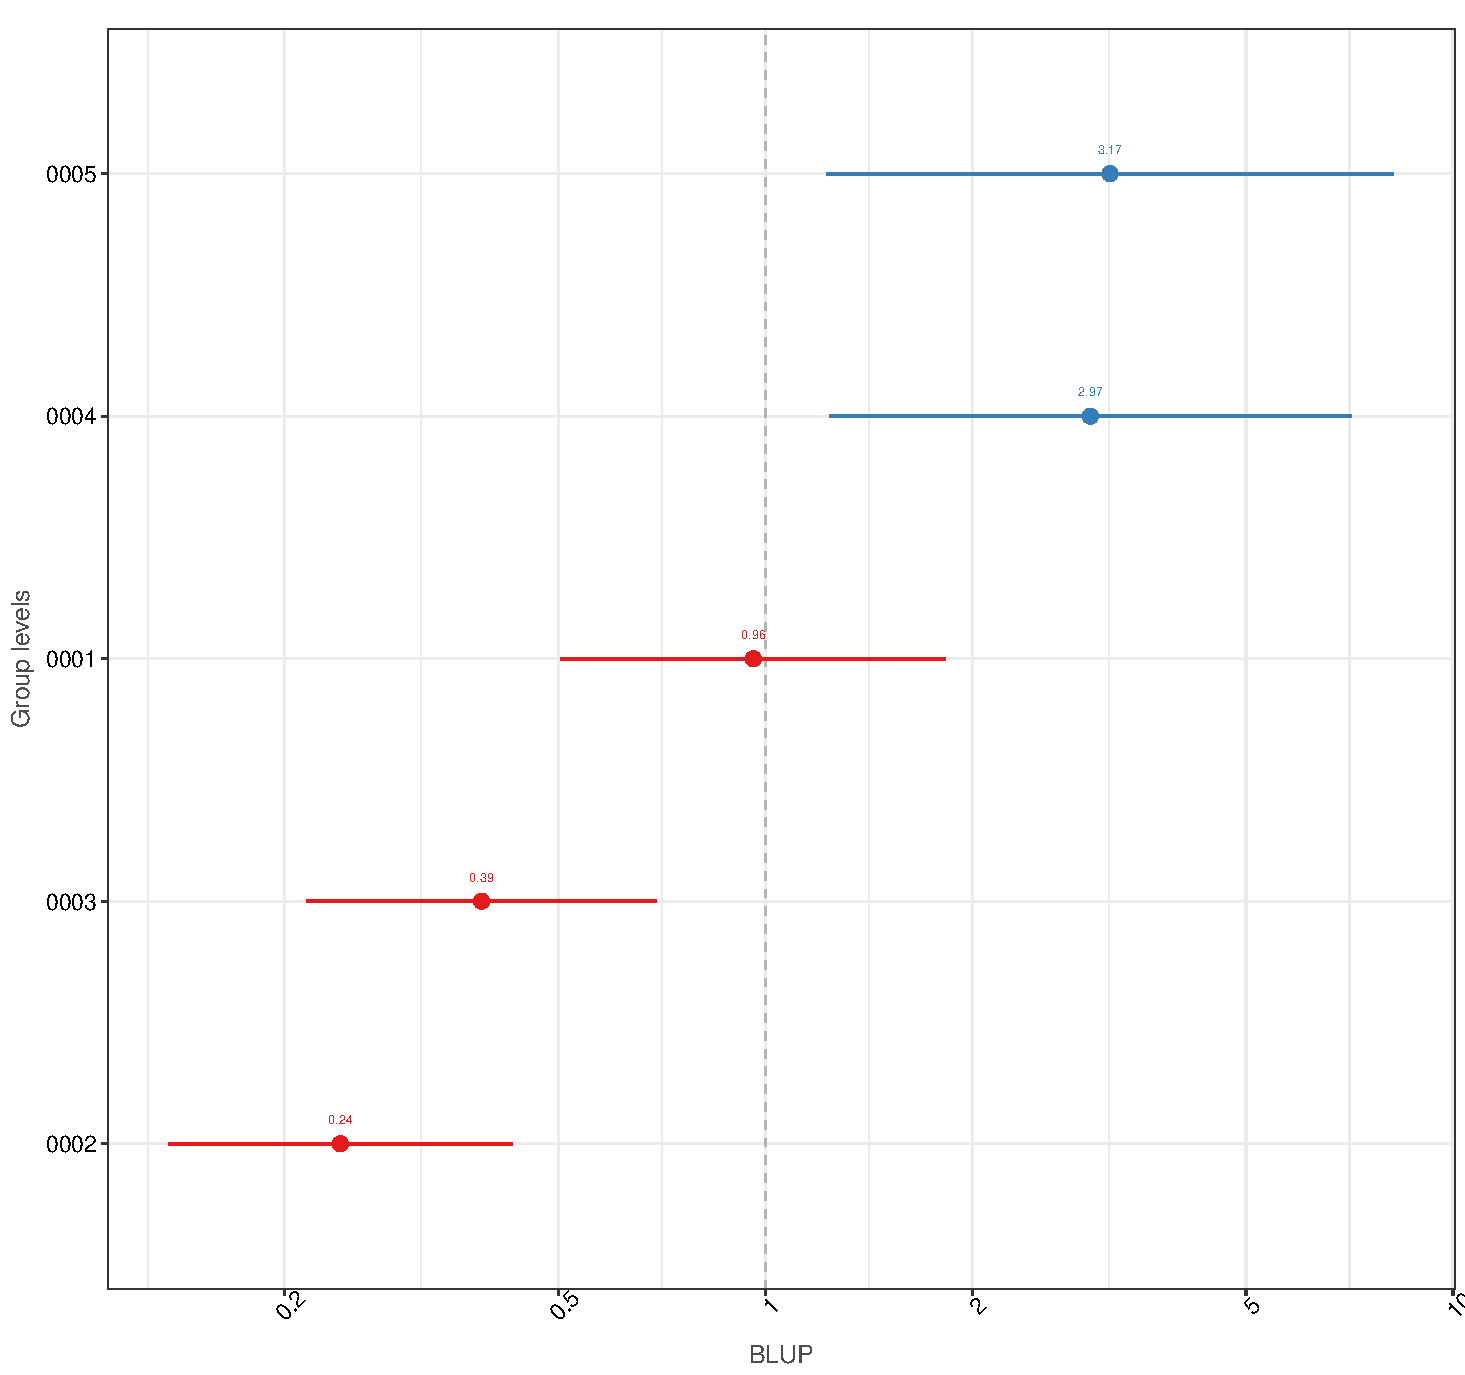
\includegraphics[width=0.9\textwidth]{graphics/blups}
%   \caption{Estimated conditional modes with confidence intervals}
%   \label{fig:blups}
% \end{figure}

\paragraph{Varying intercepts and slopes}

In the \texttt{summary} output for a VIVS model such as (\ref{eq:glmm05}), the columns \texttt{Variance} and \texttt{Corr} can be regarded as specifying the lower triangle of the variance-covariance matrix.%
\footnote{Alternatively, the \texttt{VarCorr} function could be used to extract this information.}

\vspace{0.5\baselineskip}

\begin{lstlisting}
Random effects:
 Groups Name        Variance Std.Dev. Corr 
 lemma  (Intercept) 0.6103   0.7812        
        discourse   0.8944   0.9457   -0.39
Number of obs: 2500, groups:  lemma, 50

Fixed effects:
            Estimate Std. Error z value Pr(>|z|)    
(Intercept)   0.6332     0.1226   5.163 2.43e-07 ***
discourse    -1.0428     0.1492  -6.990 2.75e-12 ***
\end{lstlisting}

This output tells us that the estimated variance in the intercepts is $\hat{\sigma}_{\alpha}^2=0.6103$, the estimated variance in the slopes is $\hat{\sigma}_{\beta}^2=0.8944$, and the covariance coefficient estimate is $\hat{\rho}=-0.39$ (a healthy value).
The means are estimated as $\hat{\mu}_{\alpha}=0.6332$ and $\hat{\mu}_{\beta}=-1.0428$.
Compare this to Section~\ref{sec:morecomplexmodels}, especially (\ref{eq:glmm06}).
It is possible to reconstruct group-wise models from this output and a lookup of the group-specific predictions using the \texttt{ranef} function.
For the first group, for example, the following can be done.

\vspace{0.5\baselineskip}

\begin{lstlisting}
ranef(alternation)$lemma[1,]
\end{lstlisting}

The output is as follows.

\vspace{0.5\baselineskip}

\begin{lstlisting}
     (Intercept) discourse
0001   0.4351156 -1.227842
\end{lstlisting}

This means that for the first lemma, actual predictions for the outcome of the alternation can be made using (\ref{eq:glmm012}), where values are rounded to two decimal digits.
Compare this to (\ref{eq:glmm05}).

\begin{equation}
  Pr(y^i=1)=logit^{-1}( [0.63+0.44] + [-1.04-1.23]\cdot x_d^i )
  \label{eq:glmm012}
\end{equation}

% \subsection{Summary and recommendations for a protocol}
% \label{sec:summaryandrecommendationsforaprotocol}
% 
% In this chapter, readers should have learned that the output of R is transparent when practitioners are able to relate it to (1) the structure of their data set and (2) the specification of the model.
% As a general protocol, it is recommended that for each study, researchers first examine their data set, then specify a model in mathematical notation \textit{including the variance-covariance matrix} based on their knowledge of the data and the theory behind their study.
% After the re-specification in R and the estimation, the R output and the model specification can be easily related, and informed inferences can be made.

\section{Representative studies}

\begin{mdframed}
  \subsection*{\citet{WolkEa2013}}
  
  \paragraph{Research questions}

  The authors aim to achieve two things.
  First, they want to compare changes in two word order related alternations in the history of English between 1650 and 1999: the dative alternation and the genitive alternation.
  They look for influencing features shared in both cases as well as construction-specific features.
  Second, they aim to show that historical data fits well into a probabilistic, cognitively oriented view of language.

  \paragraph{Data}

  The authors use the \textsc{archer} corpus, which contains texts from various registers from 1650 to 1999.
  For both constructions, carefully designed sampling protocols were used (see their Section~4).
  For the annotation of the data, both available corpus meta data were used (text ID, register, time in fractions of centuries, centered at 1800) as well as a large number of manually coded variables (constituent length, animacy, definiteness, etc.).
  Furthermore, the possessor head lemma (genitive alternation) and the verb lemma (dative alternation) were coded.

  \paragraph{Method}

  Two mixed effects logistic regression models are estimated.
  For the genitive alternation, the text ID and the possessor head lemma are used as crossed random effects.
  The authors state on p.~399 that they collapsed all head noun lemmas with less than four occurrences into one category because otherwise ``difficulties'' would arise.
  However, it is the advantage of random effects modeling that it can deal with a situation where categories have low numbers of observations (see \textit{shrinkage} in Section~\ref{sec:choosingbetweenrandomandfixedeffects}).
  For the dative alternation, the model includes the text ID, the register (which nests the text ID) as well as the lemma of the theme argument and the verb. 

  \paragraph{Results}

  It is found that many important factors have a shared importance in both alternations, \eg definiteness, animacy, construction length.
  It is also argued that the observed tendencies -- such as \textit{short-before-long} and \textit{animate referents first} -- are in line with synchronic corpus based and experimental findings about general cognitive principles underlying the framework of probabilistic grammar.
  These tendencies remain stable, but their influence strength changes over time.

\end{mdframed}

\vspace{2\baselineskip}

\begin{mdframed}

  \subsection*{\citet{Gries2015}}

  \paragraph{Research questions}
  
  The paper is programmatic in nature.
  The author re-analyses data from a previously published study on verb particle placement in English.
  He uses a GLMM instead of a fixed-effects logistic regression to show that including random effects in order to account for variation related to mode, register, and subregister increases the quality and predictive power of the model.
  He also argues that not doing so, corpus linguists risk violating fundamental assumptions about the independence of the error terms in models.
  
  \paragraph{Data}
  
  The data are $2,321$ instances of particle verbs showing either verb--direct object--particle or verb--particle--direct object order, taken from the ICE-GB.
  The grouping factors taken from the structure of the corpus are mode (only two levels), register (five levels), and subregister ($13$ levels).
  They are nested: mode nests register, which nests subregister.
  Additionally, verb and particle lemma grouping factors are annotated.
  Finally, two fixed effects candidates are annotated (the type of the head of direct object and the logarithmized length of the direct object in words).
  
  \paragraph{Method}
  
  The author uses the model selection protocol described in \citet{ZuurEa2009} to first find the optimal random effects structure using ANOVAs and AIC comparisons as well as analyses of the estimated variance for single random effects.
  He then goes on to find the optimal fixed effects structure.
  Additionally, he compares the pseudo-$R^2$ measure of the resulting mixed models.
  
  \paragraph{Results}

  It is found that the verb and particle lemma play and the subregister play a significant role.
  Notably, the variance estimate for mode is close to $0$ from the beginning of the model selection procedure.
  This is not surprising, as two levels are not nearly enough in order for the variance to be reliably estimated, and it could maybe be used as a second-level predictor for (sub)register instead.
  The $R^2$ values of the final model are very high, with a considerable difference between marginal $R^2_m=0.57$ and conditional $R^2_c=0.748$, which indicates that the random effects do in fact improve the model fit.
  It is also shown that the classification accuracy is considerably improved over that of a GLM without random effects for different lexical groups and subregisters.
  The paper thus shows that it is not appropriate to ignore lexical grouping factors and grouping factors derived from the corpus structure, especially as both are easy to annotate automatically.

\end{mdframed}

\section{Further reading}
\label{sec:furtherreading}

% This article was written in a way such that readers should be able to move on to more advanced text books written by statisticians instead of practitioners.
% There are, however, no up-to-date, comprehensive, and accessible text books written for linguists, and readers will have to live with the fact that examples in these text books are taken from political or social science, biology, etc. 
Chapters~1--15 and Chapters~20--24 of \citet{GelmanHill2006} are a highly recommended read, especially for R and \texttt{lme4} users.
Similarly, \citet{ZuurEa2009} has a reputation among R users of mixed effects models in many fields.
% Also, \cite{Fox2016} is a helpful resource.
% The non-technical passages of \citet{FahrmeirEa2013} could be considered.
The companion to \texttt{lme4}, \citet{Bates2010} and the overview in \citet{BatesEa2015} are obligatory reads for users of \texttt{lme4}.
% The GLMM FAQ collected by Ben Bolker is also a de-facto standard among R users working with GLMMs: \url{http://bbolker.github.io/mixedmodels-misc/glmmFAQ.html}

\printbibliography

\end{document} 
